\chapter{АНАЛИТИЧЕСКАЯ ЧАСТЬ}

В данном разделе будут формализованы задача и данные. Будут описаны теоретические сведения, которые нужны для решения поставленной задачи. 
\section{Протокол HTTP}\label{data}

HTTP~\cite{http}  --- это протокол, позволяющий получать различные ресурсы, например HTML-документы. Протокол HTTP лежит в основе обмена данными в Интернете. HTTP является протоколом клиент-серверного взаимодействия, что означает инициирование запросов к серверу самим получателем, обычно веб-браузером. Полученный итоговый документ будет (может) состоять из различных поддокументов, являющихся частью итогового документа: например, из отдельно полученного текста, описания структуры документа, изображений, видео-файлов, скриптов и многого другого.

HTTP --- это клиент-серверный протокол, то есть запросы отправляются какой-то одной стороной — участником обмена (user-agent) (либо прокси вместо него). Чаще всего в качестве участника выступает веб-браузер, но им может быть кто угодно, например, робот, путешествующий по Сети для пополнения и обновления данных индексации веб-страниц для поисковых систем.

Структура HTTP-сообщения всегда одинакова:

\begin{enumerate}
	\item Стартовая строка, в которой определяется адрес, по которому отправляется запрос, и тип сообщения. Указывается метод, который определяет действия при получении этого сообщения. Это может быть чтение данных, их отправка, изменение или удаление.
	\item Заголовки (Headers), в которых прописаны определённые параметры сообщения. Например, может быть напрямую задан язык.
	\item Тело запроса (Request Body), текст сообщения — данные, которые передаются. Например, файлы, отправляемые на сервер.
\end{enumerate}

\section{Сокеты}\label{functions}

Сокеты --- название программного интерфейса для обеспечения обмена данными между процессами. Процессы при таком обмене могут исполняться как на одной ЭВМ, так и на различных ЭВМ, связанных между собой сетью. Сокет --- абстрактный объект, представляющий конечную точку соединения.

Каждый процесс может создать слушающий сокет и привязать его к какому-нибудь порту операционной системы (в UNIX непривилегированные процессы не могут использовать порты меньше 1024). Слушающий процесс обычно находится в цикле ожидания, то есть просыпается при появлении нового соединения. При этом сохраняется возможность проверить наличие соединений на данный момент, установить тайм-аут для операции и т.д.

Каждый сокет имеет свой адрес. ОС семейства UNIX могут поддерживать много типов адресов, но обязательными являются INET-адрес и UNIX-адрес. Если привязать сокет к UNIX-адресу, то будет создан специальный файл (файл сокета) по заданному пути, через который смогут сообщаться любые локальные процессы путём чтения/записи из него. Сокеты типа INET доступны из сети и требуют выделения номера порта.

Обычно клиент явно подсоединяется к слушателю, после чего любое чтение или запись через его файловый дескриптор будут передавать данные между ним и сервером.

В таблице~\ref{tbl:2} представлены основные функции для работы с сокетами.

\captionsetup{justification=raggedleft,singlelinecheck=off}
\begin{table}[H]
	\centering
	\caption{Основные функции для работы с сокетами}
	\label{tbl:2}
	\begin{tabular}{|l|l|}
		\hline
		\multicolumn{2}{|c|}{Общие}	\\\hline
		Socket&	Создать новый сокет и вернуть файловый дескриптор\\\hline
		Send&	Отправить данные по сети\\\hline
		Receive&	Получить данные из сети\\\hline
		Close&	Закрыть соединение\\\hline
		
		\multicolumn{2}{|c|}{\centering{Серверные}}	\\\hline
		Bind&	Связать сокет с IP-адресом и портом\\\hline
		Listen&	Объявить о желании принимать соединения. \\&Слушает порт и ждет когда будет установлено соединение\\\hline
		Accept&	Принять запрос на установку соединения\\\hline
		
		\multicolumn{2}{|c|}{Клиентские}\\\hline
		Connect&	Установить соединение\\\hline
	\end{tabular}
\end{table}

\section{Мультиплексирование ввода/вывода}

При мультиплексировании ввода/вывода~\cite{multiplex} мы обращаемся к одному из доступных в ОС системному вызову (мультиплексору), например select, poll, pselect, dev/poll, epoll и на нем блокируемся вместо того, чтобы блокироваться на фактическом I/O вызове. Схематично процесс мультиплексирования представлен на рисунке~\ref{fig:multiplex}.

\captionsetup{justification=centering,singlelinecheck=false}
\begin{figure}[H]
	\centering
	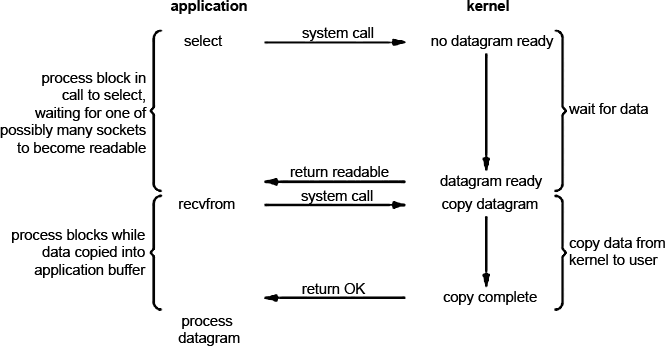
\includegraphics[width=1\linewidth]{csv/multiplex}
	\caption{Схема мультиплексированного ввода/вывода}
	\label{fig:multiplex}
\end{figure}

Приложение блокируется при вызове select'a, ожидая, когда сокет станет доступным для чтения. Затем ядро возвращает нам статус readable и можно получать данные помощью recvfrom. В отличии от блокирующего метода, мультиплексор позволяет ожидать данные не от одного, а от нескольких файловых дескрипторов. Схема работы системного вызова select изображена на рисунке~\ref{fig:select}.

\begin{figure}[H]
	\centering
	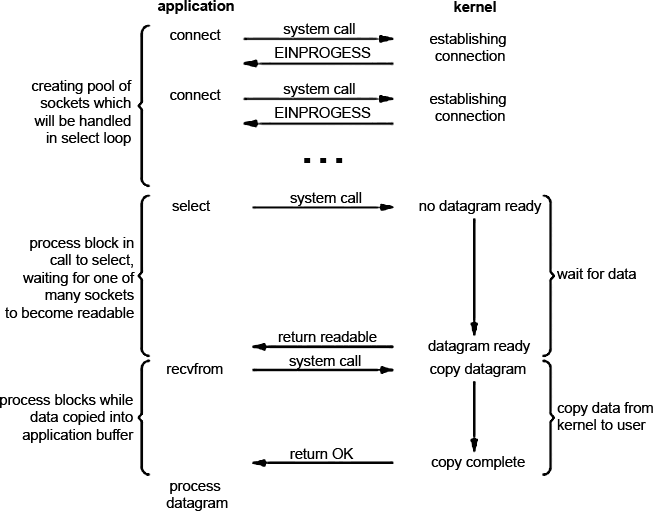
\includegraphics[width=1\linewidth]{csv/select}
	\caption{Схема работы системного вызова select}
	\label{fig:select}
\end{figure}

\section{Способ параллелизации обработки запросов}

Thread Pool поддерживает несколько потоков, ожидающих распределения задач для параллельного выполнения. Когда в систему поступает новая задача, она помещается в очередь, и один из доступных потоков в пуле забирает эту задачу на выполнение. После завершения задачи поток возвращается обратно в пул и становится доступным для выполнения новых задач. Пул потоков повышает производительность и позволяет избежать задержек в выполнении из-за частого создания и уничтожения потоков для кратковременных задач.

Prefork --- это способ параллелизации, при котором родительский процесс создаёт дочерние процессы для выполнения задач. Такой подход позволяет обрабатывать каждый запрос изолированно от остальных запросов, что повышает надежность, так как сбои в одном процессе не влияют на остальные. Однако создание процессов требует больше дополнительных ресурсов, чем использование пула потоков.


